\appendix

\section{Samplewise Convergence Inheritance}
\label{app:convergence}
This appendix records the defensive result used in the main text. It is not presented as a new MLP convergence theory.

For each $(t,x)$ let $\mathcal C(t,x)$ be nonempty, closed, and convex, let $\Pi_{t,x}$ be its metric projector, and define
\begin{equation}
\bar f(t,x,y)=f(t,x,\Pi_{t,x}y).
\label{eq:barf}
\end{equation}
Assume $(t,x,y)\mapsto\Pi_{t,x}y$ is measurable, the exact state $Y^\star(t,x)$ is feasible, $f$ is uniformly $L$-Lipschitz on $\mathcal C(t,x)$ in its state argument, and the remaining coefficient, terminal-data, moment, and random-time assumptions of the chosen gradient-dependent MLP theorem hold for $\bar f$.

\begin{proposition}[Inheritance for pointwise Samplewise IR]
Under these assumptions, $\bar f$ is globally $L$-Lipschitz in $y$, the intended feasible solution also solves the PDE with $f$ replaced by $\bar f$, and the recursion that projects each child only immediately before a driver call is pathwise identical to ordinary MLP applied to $\bar f$ on the same random tree. Hence the corresponding published convergence and complexity bounds apply to Samplewise IR under their remaining assumptions.
\end{proposition}
\begin{proof}
Metric projection is nonexpansive, so
\begin{align*}
|\bar f(t,x,y)-\bar f(t,x,y')|
&\le L\norm{\Pi_{t,x}y-\Pi_{t,x}y'}\\
&\le L\norm{y-y'}.
\end{align*}
Feasibility gives $\Pi_{t,x}Y^\star=Y^\star$, hence $\bar f(t,x,Y^\star)=f(t,x,Y^\star)$. Finally, at every finite MLP depth, replacing a child $Y$ by $\Pi_{t,x}Y$ before evaluating $f$ produces exactly the call $\bar f(t,x,Y)$. Induction on depth gives pathwise identity with ordinary MLP for $\bar f$, after which the existing theorem applies.
\end{proof}

This argument does \emph{not} cover Batch-IR because $\alpha_B$ depends jointly on siblings. It also does not cover a different algorithm that first projects samples and then averages them into a new state estimator: for nonlinear $\Pi$, generally $\E[\Pi(Y)]\neq\Pi(\E Y)$. Fixed affine/subspace projections are special because they commute with averaging.

\section{Counterexample Details and Ablations}
\label{app:counter}
\subsection{Source lower bound and certification}
Let $U^d_{n,m}$ denote the source full-history recursion and set $Y_d^\star=(u_d,\nabla u_d)$. \citet{HutzenthalerNguyen2025} show that for every $p\ge0$ and every integer $n>2p$,
\[
\liminf_{d\to\infty}d^{-p}
\left(\E\norm{U^d_{n,m}(0,0)-Y_d^\star(0,0)}^2\right)^{1/2}
=\infty.
\]
This is a depth-dependent asymptotic statement, not a claim that one fixed depth grows faster than every polynomial.

For any translation $a$ with $a_1=0$, $u_d(t,x+a)$ has the same PDE and terminal data as $u_d(t,x)$. Uniqueness gives invariance in coordinates $2{:}d$, hence $\partial_{x_j}u_d=0$ for $j\ge2$. The PDE reduces to the heat equation and
\[
u_d(t,x)=\E|x_1+\sqrt{1-t}\,G|,
\qquad G\sim\mathcal N(0,1).
\]

\subsection{Ablations}
If subspace projection is used only inside the generator but not on the returned gradient, nonlinear corrections still vanish, but the inactive final-gradient coordinates remain. At the origin,
\[
\E\norm{\widehat Y_{\rm gen-only}-Y^\star}^2
=\frac{d+3-2/\pi}{N}.
\]
If projection is applied only at the final state, the value component is unchanged realization by realization from raw MLP, because all earlier generator calls are identical.

For the first terminal block,
\begin{align*}
\E\norm{V_{\perp,N}}^2&=\frac{d-1}{N},\qquad
\E f_d(V_N)^2=\frac{d-1}{N},\\
f_d(Q_dV_N)&=0.
\end{align*}
This quantifies the first conversion of centered inactive-gradient noise into a positive nonlinear source.

\begin{figure}[t]
\centering
\IfFileExists{figures/counterexample_exact_rmse.pdf}{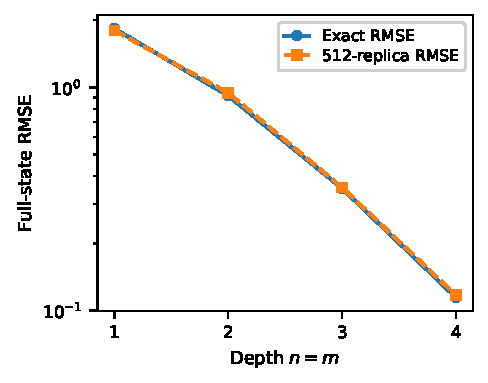
\includegraphics[width=.7\columnwidth]{figures/counterexample_exact_rmse.pdf}}{\fbox{\parbox[c][22mm][c]{.68\columnwidth}{\centering Figure asset is included in the Overleaf package.}}}
\caption{Independent Gaussian-moment validation of the exact RMSE in Theorem~\ref{thm:rescue}.}
\end{figure}

